\documentclass[times,10pt,twocolumn]{article} 
\usepackage{simpleConference}
\usepackage{times}

% Pour la commande onecolabstract (résumé 1 pleine largeur)
\usepackage{abstract}


%\usepackage[margin=2cm, columnsep=20pt]{geometry}
%\usepackage[affil-it]{authblk}
%\renewcommand{\abstractnamefont}{\normalfont\bfseries}
%\renewcommand{\abstracttextfont}{\normalfont\itshape}

% Pour les titres de section/sous-section
%\usepackage[compact]{titlesec}
%\titleformat{\section}{\large\bfseries}{\thesection}{1em}{}
%\titleformat{\subsection}{\normalsize\bfseries}{\thesubsection}{1em}{}
%\titleformat{\subsubsection}{\normalsize}{\thesubsubsection}{1em}{}


%\makeatletter
%\def\@maketitle{%
  %\newpage
  %\null
  %\vskip 2em%
  %\begin{center}%
  %\let \footnote \thanks
    %{\Large\bfseries \@title \par}%
    %\vskip 1.5em%
    %{\normalsize
      %\lineskip .5em%
      %\begin{tabular}[t]{c}%
        %\@author
      %\end{tabular}\par}%
    %\vskip 1em%
    %{\normalsize \@date}%
  %\end{center}%
  %\par
  %\vskip 1.5em}
%\makeatother

%\usepackage{xpatch}
%\xpatchbibmacro{textcite}
%{\setunit{\addcomma}\usebibmacro{cite:extrayear}}
%{\setunit{\compcitedelim}\usebibmacro{cite:labelyear+extrayear}}
%{}
%{}

\usepackage[french]{babel}
%\usepackage[T1]{fontenc}
\usepackage{lmodern}
\usepackage{csquotes}

%\usepackage[style=authoryear-comp, natbib]{biblatex}
\usepackage[style=authoryear-comp, natbib]{biblatex}
\addbibresource{bibfile.bib}
\DefineBibliographyStrings{french}{in={dans},inseries={dans}}
\renewcommand*{\bibfont}{\small}

\usepackage{amsmath}
\usepackage{amssymb}
\usepackage{mathtools}
\usepackage{amstext}
\usepackage{amsthm}
\usepackage{bbm}
\usepackage{fancyhdr}
\usepackage{siunitx}
\usepackage{physics}

\usepackage{xcolor}
\usepackage{hyperref}
\hypersetup{
    colorlinks,
    linkcolor={blue!90!black},
    citecolor={blue!90!black},
    urlcolor={blue!90!black}
}


\usepackage{graphicx}
\usepackage{float}
\graphicspath{{figures/}} %Setting the graphicspath
\usepackage{float}
\usepackage{caption}
\usepackage{subcaption}
\usepackage{tabularx}
\usepackage{dcolumn}
\usepackage{booktabs}
\usepackage{makecell}

\captionsetup{format=plain, font=small, labelfont=bf}
%\renewcommand\thesubsection{\alph{subsection})}
%\renewcommand\thesubsubsection{\Roman{subsubsection}}


\newcommand{\angstrom}{\textup{\AA}}
% Astronomy
\DeclareSIUnit\parsec{pc}
\DeclareSIUnit\lightyear{ly}


%Titre
\title{\vspace{-10mm}
\line(1,0){400}\\
Mesure de $H_0$ avec le quasar lentillé \textsc{RXJ1131-1231}
\line(1,0){400}
\vspace{-4mm}
}


%Auteur
\author{\large \textsc{Alexandre Adam}, \textsc{Charles Wilson}}
%\affil{Département de physique \\ Université de Montréal}
\affiliation{\vspace{2mm} PHY6669 -- Cosmologie\\
Département de physique \\ Université de Montréal
}
\date{\today}

\begin{document}
\twocolumn[
\maketitle
\begin{onecolabstract} % 10 points
L'étude multi-domaines du quasar quadruplement lentillé RXJ1131-1231 permet 
de déterminer la constante de Hubble à partir du formalisme de la cosmographie et 
des délais temporels. Dans cette étude, on analyse les données provenant du télescope 
de Hubble avec l'instrument ACS dans le filtre F814w pour estimer la distribution de masse 
du déflecteur du système et la distribution de la brillance de la source. Ces estimés, 
combiné avec la cosmologie $\Lambda$CDM nous permet de contraindre la constante de Hubble à 
$H_0 = 91.07^{+5.56}_{-5.26}$, soit une précision de 6\%.
\vspace{4mm} %
\end{onecolabstract}
]

\section{Introduction}\label{sec:intro}

La mesure du taux d'expansion de l'Univers $H_0$, nommé en l'honneur 
d'Edwin Hubble pour sa découverte (\citet{Hubble1929}), est un projet 
central à la cosmologie moderne. En effet, cette quantité nous informe 
autant sur la taille de l'Univers que sur l'abondance des éléments 
dans l'Univers primordial.

Les vingt dernières années ont vu la quantité et la qualités des données 
cosmologiques grandir au point où les différentes expériences sont en mesure 
de déterminer la valeur de cette constante avec une précision de quelque 
pourcentages (\citet{Riess2019}, \citet{Riess2016} et \citet{Wong2020}), 
voir moins dans le cas de la \citet{PlanckCollaboration2018}. 

Les mesures faites dans l'Univers local (relation période-luminosité 
des Céphéides, luminosité de supernov\ae de type Ia et cosmographie à 
partir de lentilles gravitationnelles) sont en tension de façon 
significative ($\sim 5\sigma$) avec les mesures faites 
dans l'univers jeune avec le fond diffus cosmologique (CMB). Cette 
crise de la cosmologie moderne est sujet de plusieurs spéculations et 
hypothèses sur la nature de cette tension. Ceci motive la recherche pour 
améliorer la précision statistique des mesures de $H_0$ local. 

Cette étude se concentre donc sur la cosmographie basé sur les lentilles 
gravitationnelles, soit l'étude des déformations géographique d'un système 
source-lentille pour déterminer l'échelle physique du système et la masse contenue 
dans la lentille. 
On s'intéresse en particulier 
au système RXJ1131-1231 qui fait partit de l'ensemble 
des lentilles utilisés par l'étude de \citet{Wong2020}. 
Cette lentille est intéressante car elle ajoute un biais statistique sur $H_0$ 
dû la valeur de la constante de Hubble inférée de ce système qui est généralement 
élevé par rapport à l'estimé de la moyenne 
statistique d'une population de lentilles 
(voir \citet{Suyu2013}, \citet{Birrer2016}).

Notre étude se concentre sur la détermination des potentiels de Fermat 
via la modélisation de la lentille et de la source avec les données provenant du 
télescope Hubble. Les délais temporels sont déterminés indépendamment par 
Charles Wilson à partir 
des données photométriques collectées par la collaboration \textsc{CosmoGrail} 
(\citet{Tewes2013}).

Les sections \ref{sec:lens} et \ref{sec:delay} se concentrent sur la 
théorie des lentilles gravitationnelles pour établir le formalisme 
qui nous permet de mesurer $H_0$. Ensuite, on discute des données 
prisent par le télescope Hubble du système RXJ1131-1231 et de la réductions 
des données \textit{a posteriori} dans la section \ref{sec:observation} 
pour faire l'inférence des paramètres 
qu'on introduit dans la section \ref{sec:inference}.
Finalement, les résultats finaux sont présentés et discuté à la section 
\ref{sec:resultats}.


%L'histoire de la cosmologie moderne trace ses débuts expérimentaux 
%avec la découverte de la 
%première galaxie par Hubble \citet{Hubble1929}, suivi de près par la 
%découverte de la loi de Hubble (\citet{Hubble1929}) qui stipule que l'Univers 
%est en expansion à un taux caractéristique $H_0$. La mesure de ce paramètre,  
%Ces observations 
%suggèrent que l'Univers est non seulement beaucoup plus vaste que l'étendue 
%de la Voie Lactée, mais qu'il doit aussi être en expansion. 

%Le succès du modèle 
%$\Lambda$CDM a expliqué ces observations mais aussi 

%L'analyse cosmographique d'une lentille gravitationnelle et des délais 
%temporelles permet d'extraire 
%L'analyse géographique d'une lentille gravitationnelle (cosmographie) permet 
%d'extraire de l'information sur le contenu de matière ainsi que les échelles de 
%distances angulaires qui donne lieu aux spectaculaires déformations de l'image de galaxies en 
%arrière plan. 
%Ce type d'analyse a gagné beaucoup de popularité durant 
%les deux dernières décennie avec la grande quantité et diversité de données collecté 
%sur ces systèmes. 


\section{Lentilles Gravitationnelles}\label{sec:lens}
\subsection{Formalisme}
Dans cette section, on révise la théorie des lentilles gravitationnelles. 
Plus de détails peuvent être trouvés dans l'excellente revue de \citet{Treu2010}. \par

Une distribution de matière projetée sur le plan normal à la ligne de visée d'un 
observateur forme ce qu'on 
appel un champ de convergence $\kappa(\boldsymbol{\theta})$, où $\boldsymbol{\theta}$ sont 
les coordonnées angulaires du plan de la lentille. Ce champ génère un potentiel 
effectif $\psi(\boldsymbol{\theta})$ lié à $\kappa$ via une équation de Poisson
\begin{equation}\label{eq:Poisson} 
        \grad^{2}_{\boldsymbol{\theta}} \psi = 2 \kappa(\boldsymbol{\theta} ).
\end{equation} 
Cette équation est résolut en introduisant la fonction de Green appropriée

\begin{equation}\label{eq:Potentiel} 
        \psi(\boldsymbol{ \theta}) = \frac{1}{\pi} \int_{\mathbb{R}^2} 
        \kappa(\boldsymbol{ \theta}') \ln(\boldsymbol{\theta} - \boldsymbol{\theta}') d^2\boldsymbol{\theta}'.
\end{equation}
Il est pratique de rendre adimensionnel les quantités d'intérêts:
\begin{equation}\label{eq:Convergence} 
        \kappa(\boldsymbol{\theta}) \equiv \frac{\Sigma(\boldsymbol{\theta})}{\Sigma_{\mathrm{cr}}},
\end{equation} 
où on a introduit la densité de surface critique $\Sigma_{\mathrm{cr}}$
\begin{equation}\label{eq:Sigcritique} 
        \Sigma_{\mathrm{cr}} \equiv \frac{c^2}{4\pi G} \frac{D_s}{D_\ell D_{\ell s}}.
\end{equation}
On distingue 3 distances de diamètres angulaires $D_s$, $D_\ell$ et $D_{\ell s}$, 
soit la distance de l'observateur à la source, à la lentille et la distance 
entre la lentille et la source respectivement. Ces distances préservent les relations 
trigonométriques entre le plan source et le plan de la lentille, ce qui donne 
lieu à l'\textit{équation de la lentille}:
\begin{equation}\label{eq:LensEquation} 
        \boldsymbol{\beta} = \boldsymbol{\theta} - \boldsymbol{\alpha}(\boldsymbol{\theta}).
\end{equation} 
$\boldsymbol{\beta}$ représente les coordonnées angulaire dans le plan de la lentille et 
$\boldsymbol{\alpha}$ représente l'angle de deflection. Comme 
$\boldsymbol{\alpha}(\boldsymbol{\theta}) = \grad_{\boldsymbol{\theta}} \psi$, alors
\begin{equation}\label{eq:DeflectionAngle} 
        \boldsymbol{\alpha}(\boldsymbol{\theta}) = \frac{1}{\pi} \int_{\mathbb{R}^{2}} \kappa(\boldsymbol{\theta}')
        \frac{\boldsymbol{\theta} - \boldsymbol{\theta}^{'}}{|\boldsymbol{\theta} - \boldsymbol{\theta}'|}
        d^{2}\boldsymbol{\theta}'.
\end{equation} 
On note 
au passage que l'équation de la lentille est linéaire par rapport à $\boldsymbol{\beta}$, 
mais non-linéaire par rapport à $\boldsymbol{\theta}$. Cet aspect devient important lorsqu'on 
cherche à optimiser la complexité numérique de la procédure d'optimisation des paramètres de la 
lentille. \par

L'équation de la lentille introduit deux effets de distortions, soit la magnification de l'image 
de la source et le cisaillement. Ces distortions sont décrites par la Jacobienne de 
l'équation de la lentille
\begin{equation}\label{eq:Jacobian} 
        A \equiv \frac{\partial \boldsymbol{\beta}}{\partial \boldsymbol{\theta}}
= \left( \mathbbm{1} - \frac{\partial^2 \psi}{\partial \theta_i \partial \theta_j} \right). 
\end{equation} 
Le cisaillement est un pseudo-vecteur $\gamma = (\gamma_1, \gamma_2)$ dans le plan de la lentille 
qui correspond à la partie antisymétrique et sans trace de la Jacobienne:
\begin{align}
        \gamma_1(\boldsymbol{\theta}) &=  \frac{1}{2} \left( \psi_{11} - \psi_{22} \right); \\
        \gamma_2(\boldsymbol{\theta}) &= \psi_{12} = \psi_{21}.
\end{align}
Ainsi, on peut modéliser les perturbations extrinsèques au déflecteur principal de la lentille 
en introduisant le potentiel extrinsèques qui correspond à un 
cisaillement constant:
\begin{equation}\label{eq:gamma_ext} 
        \psi_{\mathrm{ext}}  = \frac{1}{2} \gamma_{\mathrm{ext}} \theta^2 
        \cos 2(\varphi - \phi_{\mathrm{ext}}).
\end{equation} 
$\psi_{\mathrm{ext}}$ est exprimé en terme des coordonnées polaires du plan de la lentille 
$\boldsymbol{\theta} = (\theta, \varphi)$.

%La magnification correspond à l'inverse du déterminant de la Jacobienne. 
%\begin{equation}\label{eq:Magnification} 
        %\mu \equiv \det{A}^{-1}.
%\end{equation} 
%Cette quantité peut être utilisé pour contraindre la luminosité de noyau actif de la galaxie 
%source (AGN) via le ratio du flux des 4 images de l'AGN. Dans notre cas, 
%Les valeurs 
%propres de la matrice de cisaillement sont $\pm \sqrt{\gamma_1^2 + \gamma_2^2 } = \pm \gamma$, 
%ainsi il est plus pratique d'introduire le cisaillement en coordonnée polaires $(\gamma, \phi)$:
%\begin{equation}\label{eq:JacobianDecomposition} 
        %A = (1 - \kappa)\mathbbm{1}
        %+ \gamma R(\phi).
%\end{equation} 


\subsection{Paramétrisation}
On paramétrise la densité surfacique de la lentille par un profil elliptique avec une loi 
de puissance adoucie:
\begin{equation}\label{eq:Kappa} 
        \kappa(\boldsymbol{\theta}) = \frac{3 - \gamma'}{2} 
        \left( 
                \frac{\theta_E}{\sqrt{\theta_1^2 + \theta_2^2/q^2 + \theta_c^2}}
\right)^{\gamma'- 1}. 
\end{equation} 
$\gamma'$ est la pente logarithmique radiale du profile, $q$ est le ratio des axes 
et $\theta_E$ est le rayon d'Einstein de la lentille. On introduit le rayon du c{\oe}ur 
du profile 
$\theta_c$ pour éviter l'instabilité numérique du profile à l'origine du système de coordonnée. 
Il est pratique de fixer sa valeur à un angle plus petit que la taille angulaire d'un 
pixel de l'image (dans notre cas $\theta_c < 0.04''$). \par

%Ce choix est informé par le fait que la lentille RXJ1131-1231 exhibite 4 images, ce qui 
%survient seulement lorsque le champ de convergence est elliptique.

Les intégrales \eqref{eq:Potentiel} et \eqref{eq:DeflectionAngle} ont une solution analytique 
seulement lorsque $\gamma'= 2$ (profil isotherme elliptique) ainsi que certains autres cas 
détaillés par \citet{Keeton2001}. En première approximation, ce paramètre peut être fixé 
à $2$ sachant que la plupart des systèmes de lentilles sont bien modélisé par ce profil. 
Laisser ce paramètre complètement libre requiert de procéder avec le traitement de 
\citet{Barkana1998} ou \citet{Tessore2015}, où les intégrales pour le potentiel $\psi$ 
et les angles de déflections $alpha$ 
sont simplifiées en intégrales unidimensionnelles. \par

On choisit une solution intermédiaire valide lorsque l'ellipticité de la lentille est 
petite (voir \citet{Barkana1998}). Le profil \texttt{SPEP} suppose que la forme 
du potentiel $\psi$ est identique à celle d'un profile isotrope (où 
les intégrales ont des solutions analytiques). Les angles de déflections 
ont ainsi une forme analytique. Cette simplifications vient 
au prix de développer des isocontours dans le potentiel $\psi$
en forme d'haltères lorsque 
l'ellipticité du profil de masse s'éloigne du domaine de validité.

Le cisaillement extrinsèque est aussi ajusté lors de l'étape d'inférence. Le centre 
du champ de distortions est fixé au centre de l'image \texttt{ACS}, ce qui laisse 
les paramètres $\gamma_{\mathrm{ext}}$ et $\phi_{\mathrm{ext}}$ de l'équation 
\eqref{eq:gamma_ext} à déterminer.


%On choisit une solution intermédiaire informée du fait que la pente logarithmique 
%est très près d'une pente isotherme. Ainsi, on peut considérer une expansion de Taylor 
%au premier ordre autour de la solution isotherme. Cette approche à l'avantage d'être à 
%l'avantage d'être plus rapide à calculer numériquement. On doit toutefois restreindre 
%le domaine des valeurs possibles de $\gamma'$ à l'intervalle $\[1.6, 2.4\]$ où 
%l'erreur par rapport à la solution de Barkana 

\section{Délai temporel}\label{sec:delay}
Le delai temporel est une mesure de la différence entre le temps d'arrivé d'une image $i$ 
et une seconde image $j$ de l'AGN. Le formalisme des délai temporels d'une 
lentille gravitationnelle fut initialement introduit par \citet{Refsdal1964}. La même 
année, \citet{Shapiro1964} introduisait l'effet de dilation temporelle expérimenté par 
un photon traversant un champ gravitationnel. Les deux effets sont combinés pour 
former le potentiel de Fermat:
\begin{equation}\label{eq:PotentielFermat} 
        \Psi_{\mathrm{Fermat}} = \frac{(\boldsymbol{\theta} - \boldsymbol{\beta})^{2}}{2}
        - \psi(\boldsymbol{\theta}).
\end{equation} 
Le délai entre deux images ($i$ et $j$) est donc mesuré par l'équation

\begin{equation}\label{eq:TimeDelay} 
        c \Delta t_{ij} = D_{\Delta t} \left( \Psi_{\mathrm{Fermat, i}} - 
        \Psi_{\mathrm{Fermat, j}} \right),
\end{equation} 
où $D_{\Delta t}$ est la distance caractéristique du délai temporel
\begin{equation}\label{eq:Ddt} 
        D_{\Delta t} \equiv (1 + z_{\ell}) \frac{D_\ell D_s}{D_{\ell s}} \propto H_0^{-1}.
\end{equation}

La dégénérescence de masse peut affecter la valeurs mesurées de $D_{\Delta t}$: 
une surdensité de halos de matière noire dans la ligne de visée produit une 
distance caractéristique plus petite que la \textit{vrai} distance $D_{\Delta t}$
\begin{equation}\label{eq:Degenerescence} 
        D_{\Delta t} = \frac{D_{\Delta t}^{\text{modèle}}}{1 - \kappa_{\mathrm{ext}}}.
\end{equation} 
où $D_{\Delta t}^{\text{modèle}}$ est estimé directement à partir de l'équation 
\eqref{eq:TimeDelay}. Un estimé indépendant de la densité de 
masse extrinsèque au plan 
de la lentille $\kappa_{\mathrm{ext}}$ 
permet de lever cette dégénérescence.

Pour déterminer directement les délais temporels $\Delta t_{ij}$, 
\citet{Tewes2013} ont mesuré le flux photométrique des 4 images du quasar à 
tous les 4-5 jours en moyenne durant 9 ans avec 3 télescopes terrestres de 
1-2 mètres d'ouverture. Comme ces courbes de lumières sont générées par un même objet (AGN), 
les sursauts intrinsèque de luminosités sont clairement identifiables dans chaque courbe, de 
sortes que les délais temporels propre à la lentille peuvent être mesurés indépendamment. 

Pour notre analyse, on utilise les résultats obtenu par Charles Wilson avec le 
module \texttt{Pycs3} (\citet{Millon2020}). On réfère à son rapport pour une explication 
plus détaillée de la méthode employée et des sources possibles d'erreurs.

\begin{table}[H]
        \centering
        \begin{tabular}{ccc}
                \toprule
                $\Delta t_{\mathrm{BA}}$ & $0.5 \pm 5.7$ jours \\\midrule
                $\Delta t_{\mathrm{BC}}$ & $-0.3 \pm 5.5$ jours \\\midrule 
                $\Delta t_{\mathrm{BD}}$ & $92.3 \pm 7.4$ jours \\\bottomrule
        \end{tabular}
        \caption{Mesure des délais temporels.}
        \label{tab:TimeDelay}
\end{table}

%\section{Méthodologie}\label{sec:metho}
%\subsection{}
\section{Observations de RXJ1131-1231}\label{sec:observation}
La lentille gravitationnelle RXJ1131-1231 a été découverte par 
\citet{Sluse2003}. Des mesures spectroscopiques ont permis de déterminer le 
décalage vers le rouge de la source $z_s = 0.658$ et de la lentille 
$z_\ell = 0.295$ (\citet{Sluse2003}). Dans les prochaines sections, on détail 
la prise de mesure et le traitement \textit{a posteriori} des mesures pour 
extraire les données pertinentes à l'inférence.
\begin{figure}[H]
        \centering
        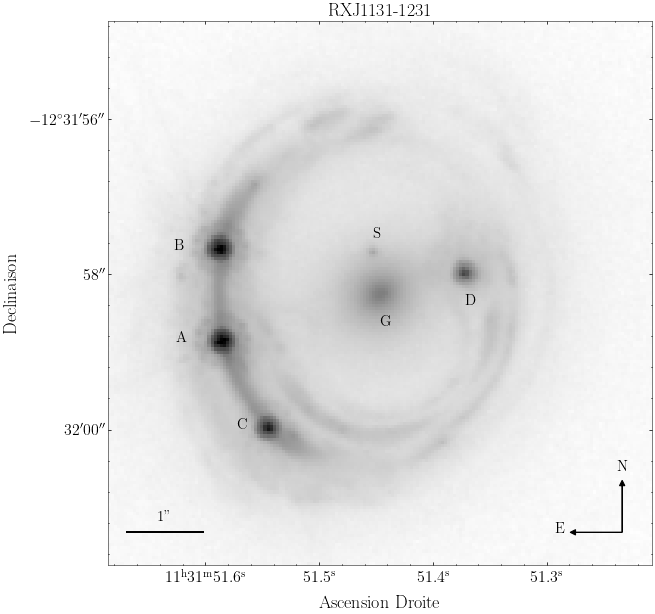
\includegraphics[width=\linewidth]{good_cutout}
        \caption{Image ACS \textit{drizzled} du système RXJ1131-1231 avec le filtre F814w obtenu 
                à partir de l'archive du télescope \textit{Hubble}. Les 
        4 images du quasar sont identifiés par les lettres A à D. Le déflecteur principal (G) 
        et son satellite (S) sont aussi identifiés. Les axes sont étiqueté par le système 
        de coordonnée céleste J2000.}
        \label{fig:rxj1131}
\end{figure}

\subsection{Traitement de l'image}
La prise de mesure consiste en 5 expositions de 1980.0 secondes avec 
l'instrument \texttt{ACS} du téléscope Hubble et le filtre F814w. Ces 
expositions sont combinées par l'algorithme \texttt{MultiDrizzle} 
(voir \citet{Massey2010} et \citet{Koekemoer2007}) à une taille angulaire 
par pixel de $0.04''$. L'image de RXJ1131-1231 (figure \ref{fig:rxj1131}) 
est une découpe de 175 pixels de côté centré sur la position 
J2000: $11^{\mathrm{h}}31^{\mathrm{m}}51.45^{\mathrm{s}}$, $-12^{\circ}31'58.28''$.

\begin{table}[H]
        \centering
        \begin{tabular}{ccc}
                \toprule
                & \thead{$\theta_x$  [$''$]} & \thead{$\theta_y$ [$''$]} \\\midrule\midrule
                B & $2.10$ & $0.56$ \\\midrule
                A & $2.07$ & $-0.62$ \\\midrule
                C & $1.47$ & $-1.74$ \\\midrule
                D & $-1.12$ & $0.25$ \\
                \bottomrule
        \end{tabular}
        \caption{Positions des images du quasar relatives au centre de l'image ACS avec 
        une incertitude commune égale à la taille angulaire d'un pixel: $0.04''$.}
        \label{tab:PositionImage}
\end{table}

Le bruit du compte d'électron dans chaque pixel
est modélisé à partir de l'image ACS et  
l'image de poids $w_{i} = 1/\sigma^2_{i}$. 
Ces poids sont 
calculé lors du processus de 
\textit{drizzling} pour tenir compte de la corrélation du bruit de chaque pixel 
avec ses voisins (voir par exemple \citet{Casertano2000}).
%La corrélation émerge 
%lors du rééchantillionnage de l dans une grille de pixels 
%effectifs.
Ces poids tiennent aussi compte  
du fond noir du ciel, du courant noir du détecteur et des pixels saturés 
durant l'exposition (ainsi que des masques appliqués aux rayons cosmiques 
et traces laissées par des satellites).
Le bruit effectif est donc l'addition en quadrature du bruit de Poisson de 
l'image ACS et des poids 
{($\sigma_{\mathrm{ACS}, i} = \sqrt{d_{\mathrm{ACS}, i} + \sigma^2_i}$)}.



La lumière des galaxies G et S est décomposé de l'image ACS pour 
isoler le système lentillé. Pour ce faire, on utilise le 
logiciel \texttt{GalFit} (\citet{Peng2002,Peng2010}). On trouve que la 
galaxie G est bien modélisé par deux profils de Sérsic elliptique (\citet{Sersic1968}):
\begin{equation}\label{eq:} 
        \Sigma(\theta_1, \theta_2) = \Sigma_e \exp \left\{ -\kappa 
\left[  
                \left( 
                        \frac{\sqrt{\theta_1^2 + \theta_2^2/q^2}}{R_e}
         \right)^{1/n} 
         -1
\right]
 \right\},
\end{equation} 
où $\Sigma_e$ est la brillance de surface, $n$ est la pente logarithmique et 
$R_e$ est le rayon effectif du profil.
Cette procédure est commune 
(voir par exemple \citet{Suyu2013})
pour une galaxie elliptique 
avec un bulbe \textit{classique}, modélisée par 
un profil de de Vaucouleurs ($n=4$, \citet{DeVaucouleurs1948}).
Similairement, un disque \textit{classique} est modélisé par 
un profil exponentiel ($n=1$). La taille du satellite S est suffisamment petite 
qu'on choisit d'utiliser la fonction d'étalement du point (PSF) pour la 
modéliser.




La fonction d'étalement du point est extraite des objets non-résolus dans le
champ d'étoile 
avoisinant ($\simeq 2'$) au système RXJ1131-1231. 
On identifie 3 candidats potentiels (voir figure \ref{fig:psf}). 
Le candidat numéro 1 contient un anneau secondaire 
typique d'une tache d'Airy et est donc choisit pour les analyses subséquentes. 
On extrait une image de 39 pixels de côté centré sur la position de l'objet 1, 
qu'on normalize 
après avoir 
multiplié par une fenêtre de Hann (aussi connue comme \textit{Hanning window})
pour mitiger les effets de bord du découpage.

\begin{figure}[H]
        \centering
        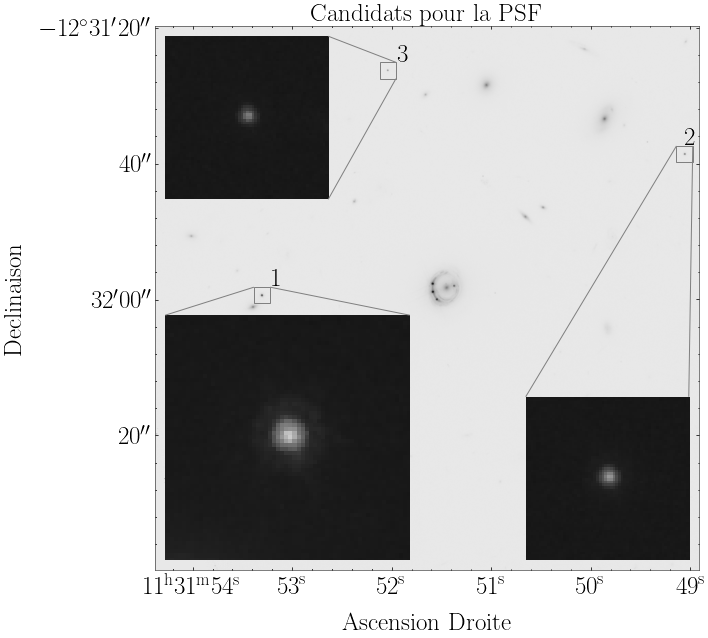
\includegraphics[width=\linewidth]{psf_cutout}
        \caption{ Sélection d'une PSF pour la reconstruction d'image dans le champs 
                d'étoile avoisinant le système RXJ1131-1231 (visible au centre 
                de l'image). Le candidat 1 (coin sud-est de l'image) contient 
                un anneau secondaire typique d'une tache d'Airy.
        }
        \label{fig:psf}
\end{figure}


\begin{figure*}[ht]
        \centering
        \begin{subfigure}[b]{0.45\linewidth}
                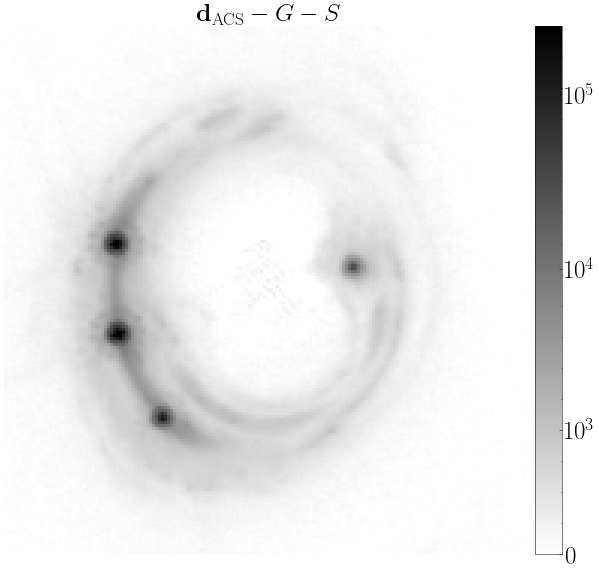
\includegraphics[width=\linewidth]{after_galfit} 
                \caption{
                %Soustraction des profils de brillance des galaxies G et S.
        }
                \label{fig:after_galfit}
        \end{subfigure}
        ~
        \begin{subfigure}[b]{0.48\linewidth}
                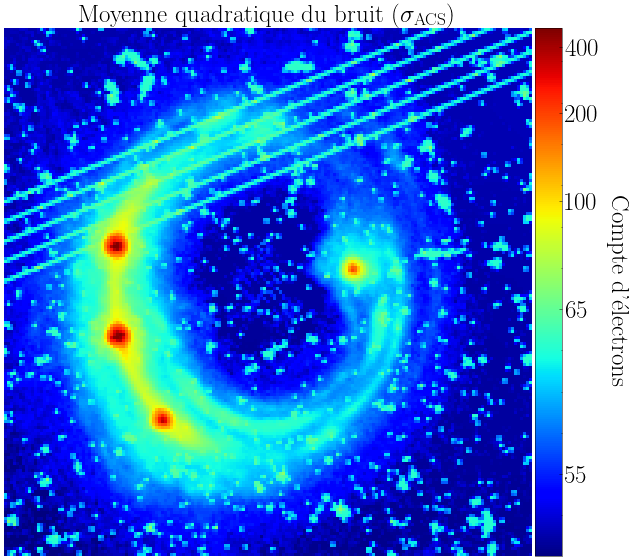
\includegraphics[width=\linewidth]{noise_map}
                \caption{
                        %Addition en quadrature de l'image de poids et du bruit de 
                %Poisson.
        }
                \label{fig:noise_map}
        \end{subfigure}
        \caption{Prétraitement de l'image et modélisation du bruit.}
\end{figure*}
%Les délai temporels sont donc déterminé via la translation temporelle de ces courbes 
%tels que ces sursauts correspondent un à l'autre, donné un
%%La procédure de maximisation de la vraisemblance de la translation temporelle de ces 
%courbes permet d'identifier directement les délais temporels propre au système de lentille 
%et la masse projeté dans le cône de lumière entre l'observateur et la source.


\subsection{Convergence extrinsèque}
\citet{Suyu2013} ont observé RXJ1131-1231 avec le \textit{Low-Resolution Imaging 
Spectrometer} (\citet{Oke1995}) installé sur Keck I 
pour estimer la vélocité de dispersion de la galaxie lentille G projetée 
selon la ligne de visée. Les deux premiers moments de la vélocité
de dispersion sont estimés via une simulation MCMC du spectre de la galaxie 
et un ajustement aux observations.

%Une analyse détaillé de la cinématique stellaire permet en principe de contraindre 
%certains paramètres de la lentille indépendamment des halos de matières noires dans 
%le cône de visée entre l'observateur et la source. Voir par exemple 
%\cite{Birrer2016}. 

Cette observation, combinée à un compte statistique 
des galaxies avoisinant le système lentillé (\citet{Fassnacht2011}), permet d'estimer 
la convergence extrinsèque au plan de la lentille. On estime ses trois premiers 
moments à partir des résultats de \citet{Suyu2013} (figure 6 de l'article), 
soit la moyenne $\mu_{\kappa}=0.1$, la déviation standard $\sigma_\kappa=0.042$ et 
l'asymétrie $\gamma_\kappa=0.8$.


\section{Inférence}\label{sec:inference}
Pour l'inférence des paramètres de la lentille, de la source et 
de la distance caractéristique du délai temporel, on choisit d'utiliser 
le module \textit{open-source} \texttt{Lenstronomy} (\cite{Birrer2018}). Dans 
la section suivante, on résume la théorie de probabilité sur laquelle 
la modélisation est basée ainsi que la forme des termes de vraisemblances.

\subsection{Inférence jointe}
L'inférence jointe des paramètres du modèle de la lentille $\mathcal{M}$, 
du modèle de la source $\mathcal{S}$ et de la distance caractéristique 
du délai temporel $D_{\Delta t}$ est fait à partir d'un échantillonnage 
de la distribution \textit{a posteriori} 
$P(D_{\Delta t}, \mathcal{M}, \mathcal{S} \mid \Delta t_{1:3}, 
\boldsymbol{d}_{\mathrm{ACS}}, \boldsymbol{\theta}^{\mathrm{AGN}}_{1:4})$. 
On adopte le point de vue de Bayes pour estimer cette distribution 
à partir de 3 termes de vraisemblances ainsi que des distributions 
\textit{a priori} des paramètres 
qu'on suppose indépendantes (donc séparable):
\begin{align}\label{eq:Bayes} 
        \nonumber
        P(D_{\Delta t}, &\mathcal{M}, \mathcal{S} \mid 
\Delta t_{1:3}, 
\boldsymbol{d}_{\mathrm{ACS}}, \boldsymbol{\theta}^{\mathrm{AGN}}_{1:4}) \propto \\ 
\nonumber
&P(\boldsymbol{\theta}^{\mathrm{AGN}}_{1:4} \mid \mathcal{M}, \boldsymbol{\beta}^{\mathrm{AGN}})
P(\mathbf{d}_{\mathrm{ACS}} \mid \mathcal{M}, \mathcal{S}) \\
&P(\Delta t_{1:3} \mid D_{\Delta t}, \mathcal{M})P(\mathcal{M})P(\mathcal{S})P(D_{\Delta t})
P(\boldsymbol{\theta}^{\mathrm{AGN}}_{1:4})
\end{align}
où $\boldsymbol{\beta}^{\mathrm{AGN}} \in \mathcal{S}$. 

Cette approche nous permet d'adopter l'algorithme MCMC,
implémenté dans \texttt{EMCEE} 
(\citet{Foreman-Mackey2013}) avec la proposition invariante affine 
de \citet{Goodman2010}, pour estimer la distribution 
\textit{a posteriori} autour d'un maximum qu'on doit
déterminer auparavant à l'aide d'un algorithme de recherche de maximum 
comme le \textit{Particle Swarm Optimizer} (PSO, \citet{Eberhart1995}) 
implémenté dans 
\texttt{Lenstronomy}. 

On doit aussi, avec plusieurs essais-erreurs, 
estimer le point 
de départ des paramètres pour l'algorithme PSO qui n'est pas garantit 
de converger au maximum absolu. 
On note que le choix du point de départ 
pour les paramètres a pour 
effet de régulariser indirectement 
%(ajout d'une distribution \textit{a priori} sur les paramètres) 
la distribution \textit{a posteriori}. Le choix final est 
rapporté dans la table \ref{tab:results}.

Cette approche est préférée au \textit{Nested Sampling} implémentée 
dans \texttt{Dynesty} (\citet{Skilling2006}, \citet{Higson2017}) adoptée 
précédemment pour un modèle plus simple. Bien que cette seconde méthode est 
plus précise en principe, 
elle requiert beaucoup plus d'évaluation des vraisemblances pour 
explorer tout le volume de la distribution \textit{a priori} pour estimer 
l'évidence $\mathcal{Z}$. 

Une fois le maximum trouvé, l'algorithme MCMC est idéalement exécuté 
pour un nombre d'itérations suffisamment élevé pour permettre aux 
marcheurs aléatoires d'atteindre un état ergodique. Cette analyse requiert 
un estimé du temps d'autocorrélations des chaînes pour chaque paramètres 
(\cite{Goodman2010}). On rapporte cette valeur seulement 
pour $D_{\Delta t}$ dans la 
figure \ref{fig:mixing}.
%l'algorithme \texttt{MCMC} est exécuté 
%plusieurs fois, chaque fois avec une position de départ près du maximum 
%estimé à l'étape précédente
%et un nombre d'itération suffisamment grande pour que les marcheurs aléatoires 
%puisse satisfaire l'hypothèse ergodique. 
%Cette procédure a pour objectif d'augmenter la résolution de la distribution 
%autour du maximum et estimer une incertitude valide des paramètres d'intérêts.

\subsection{Vraisemblances}
Par supposition, les 4 images du quasar proviennent de la même position 
dans le plan source jusqu'à une certaine tolérance $\sigma_\beta$ 
qu'on définit comme 
un dixième de la taille d'un pixel dans l'image ACS.
Ceci motive le terme de vraisemblance 
\begin{align}
        \nonumber
        \log P(\boldsymbol{\beta}^{\mathrm{AGN}} &\mid \mathcal{M}, 
        \boldsymbol{\theta}^{\mathrm{AGN}}_{1:4}
        %\underbrace{\theta_E, \gamma', q, \phi, \theta_{x, 0}, \theta_{y, 0}}_{\mathcal{M}}) 
        )
        \propto  \\
\label{eq:SourceLike} 
        &-\frac{1}{2} \sum_{i < j}^{4} 
        \frac{\left( 
                        \boldsymbol{\beta}(\boldsymbol{\theta}_i^{\mathrm{AGN}}) - 
                        \boldsymbol{\beta}(\boldsymbol{\theta}_j^{\mathrm{AGN}})
        \right)^2}{\sigma^2_{\beta}}.
\end{align} 
où on note l'ensemble des paramètres de la lentille 
$\mathcal{M} = \{\theta_E,\, \gamma',\, q,\, \phi,\, \boldsymbol{\theta}_0,\, 
\gamma_{\mathrm{ext}},\, \phi_{\mathrm{ext}}\}$ où $\phi$ et 
$\boldsymbol{\theta}_0$ correspondent à l'orientation de l'axe principale et 
au centre du champ de convergence respectivement.
Cette vraisemblance ne contraint pas la position de la source 
$\boldsymbol{\beta}^{\mathrm{AGN}} = \overline{\boldsymbol{\beta}(
\boldsymbol{\theta}^{\mathrm{AGN}}_{1:4}})$ à 
correspondre à un point intérieur à 
la caustique tangentielle du modèle de la lentille. 
On doit donc vérifier \textit{a posteriori} 
que la position du quasar 
prédite par le modèle produit 
4 images dans le plan de la lentille.

Comme la position des 4 images du quasar est incertaine, on doit introduire un 
paramètre de nuisance $\epsilon_{1:4} \sim \mathcal{N}(0, \mathbbm{1} d \boldsymbol{\theta}^2)$ 
qui perturbe les positions $\boldsymbol{\theta}^{\mathrm{AGN}}_{1:4}$ 
autour de leur valeurs mesurés (avec \texttt{DAOStarFinder} de \citet{Stetson1987}) 
durant l'inférence. Ce paramètre est marginalisé lors de l'extraction des résultats.

Les données provenant de l'image $\mathbf{d}_{\mathrm{ACS}}$ apportent 
un ensemble de contraintes supplémentaires aux paramètres de la lentille $\mathcal{M}$ 
via la forme de l'anneau d'Einstein. Ces données permettent aussi d'ajuster 
un modèle 
formel pour la source (deux profils de Sérsic et un quasar qui partagent 
la même position) qu'on note par l'ensemble 
$\mathcal{S}$. Comme le compte d'électron dans chaque pixel considéré atteint 
une valeur suffisamment élevé, le bruit de Poisson tend à être distribué selon 
une distribution 
gaussienne et donc 
\begin{align}
        \nonumber
        \log P(\underbrace{\mathbf{d}_{\mathrm{ACS}}}_{\mathcal{D}}
        &| \mathcal{M},\, \mathcal{S}) \propto  \\
\label{eq:ImageLike}
        &-\frac{1}{2}\sum_{i=1}^{|\mathcal{D}|} \frac{(d_{\mathrm{ACS},i} - 
        d_i(\mathcal{M}, \mathcal{S}))^{2}}
        {\sigma_{\mathrm{ACS},i}^2},
\end{align} 
où 
\begin{equation}\label{eq:d_i} 
        \mathbf{d}(\mathcal{M}, \mathcal{S}) = 
        \Pi * \mathbf{L}_{\mathcal{M}}(\mathcal{S}) + 
        \Pi * \sum_{i=1}^{4}\mathbf{a}_i(\boldsymbol{\theta}_i^{\mathrm{AGN}}).
\end{equation} 
On a définit l'opérateur de la lentille comme $\mathbf{L}_{\mathcal{M}}$ et 
la fonction d'étalement du point comme $\Pi$. 
%La convolution $*$ est performée 
%dans l'espace de Fourier avec l'algorithme FFT de \texttt{Numpy}.
Pour accélérer cette partie de l'inférence, on applique un masque aux données 
pour ne sélectionner que les pixels qui ont un signal-sur-bruit d'au moins 2. On sélectionne 
ainsi $|\mathcal{D}| = 10523$ pixels sur les $175^2$ pixels de l'image ACS. 

%Aussi, 
Comme $\mathcal{S}$ est un modèle analytique, la stratégie pour calculer l'intensité 
$\mathbf{L}_{\mathcal{M}}(\mathcal{S})$ 
est de performer l'équation \eqref{eq:LensEquation} 
pour une grille de points $\boldsymbol{\theta}_{:|\mathcal{D}|}$ 
et calculer la réponse du modèle 
directement à partir des points $\boldsymbol{\beta}_{:|\mathcal{D}|}$ obtenus. 
Cette approche est 
beaucoup plus rapide et stable 
que de performer le tracé des rayons lumineux dans 
la direction inverse. 

Le terme de vraisemblance des délai temporels fait utilisation de 
l'équation \eqref{eq:TimeDelay} et des résultats de la table 
\ref{tab:TimeDelay}:
\begin{align}
        \nonumber
        \log P(\Delta t_{1:3}&| D_{\Delta t}, \mathcal{M}) \propto  \\
        \label{eq:TimeDelayLike}
                       &-\frac{1}{2} \sum_{i=1}^{3} \frac{(\Delta t_i - 
        \Delta t(D_{\Delta t}, \Delta\Psi_{\mathrm{Fermat, i}}))^{2}}{\sigma_{\Delta t, i}^{2}}.
\end{align}

\section{Résultats et discussion}\label{sec:resultats}
Les contraintes estimées lors de l'estimation MCMC des distributions 
\textit{a posteriori} ou durant l'optimisation avec \texttt{GalFit} 
sont présentés dans la table \ref{tab:results}. On ne présente que 
les résultats lié à géographie de la lentille. Pour une 
analyse de la photométrie du système, le lecteur peut se référer au 
travail de \citet{Suyu2013} et \citet{Tewes2013}.

Pour ce travail, on utilise un point de référence différent de celui utilisé 
par \citet{Suyu2013}. Les paramètres comparés dans la table \ref{tab:results} 
sont seulement ceux qui ne dépendent pas du système de coordonnées.

On doit noter la valeur du rayon d'Einstein qui diffère largement de celle 
reporté par \citet{Suyu2013}. En principe, ce paramètre est assez indépendant 
et bien ajusté par l'anneau d'Einstein du système. Notre valeur est en accord 
avec le travail plus récent de \citet{Birrer2016} qui utilise le même 
module pour ajuster les paramètres de la lentille sur les données. Cette analyse 
note que la taille angulaire du bulbe de la source joue un rôle important sur les 
paramètres estimés et leurs biais statistique. Notre analyse diffère de façon cruciale 
de celle 
de \citet{Suyu2013} au niveau de la forme assumée pour la source. Où nous utilisons 
un modèle paramétrique, \citet{Suyu2013} utilisent une reconstruction pixellisée 
(non-paramétrique) de la source. 

Les potentiels de Fermat et la distance caractéristique $D^{\text{modèle}}_{\Delta t}$ sont 
marginalisé de l'ensemble de paramètres et présentés dans la figure 
\ref{fig:special}. On rapporte les trois premiers moments de la distribution 
des potentiels de Fermat dans la table \ref{tab:Fermat}. Ces résultats 
sont utilisés pour faire abstraction des modèles $\mathcal{M}$ et $\mathcal{S}$ 
et permettre à Charles Wilson de reproduire nos résultats.

\begin{table}[H]
        \centering
        \begin{tabular}{cccc}
                \toprule
                (arcsec$^{2}$)  &  Moyenne & Déviation standard & Asymétrie \\\midrule
                $\Delta \Psi^{\mathrm{BA}}_{\mathrm{Fermat}}$ 
              & $0.01626$ & $7.05 \times 10^{-5}$  & $0.0385$ \\[1ex]
              $\Delta \Psi^{BC}_{\mathrm{Fermat}}$ 
              & -0.00381 & $1.70 \times 10^{-5}$ & $-0.0673$\\[1ex]
              $\Delta \Psi^{BD}_{\mathrm{Fermat}}$ & $2.0371$ & $0.00824$ & $0.0334$ \\
              \bottomrule
        \end{tabular}
        \caption{Trois premier moments de la distribution marginalisée des potentiels 
        de Fermat mesurés (voir figure \ref{fig:special}).}
        \label{tab:Fermat}
\end{table}

\begin{figure}[H]
        \centering
        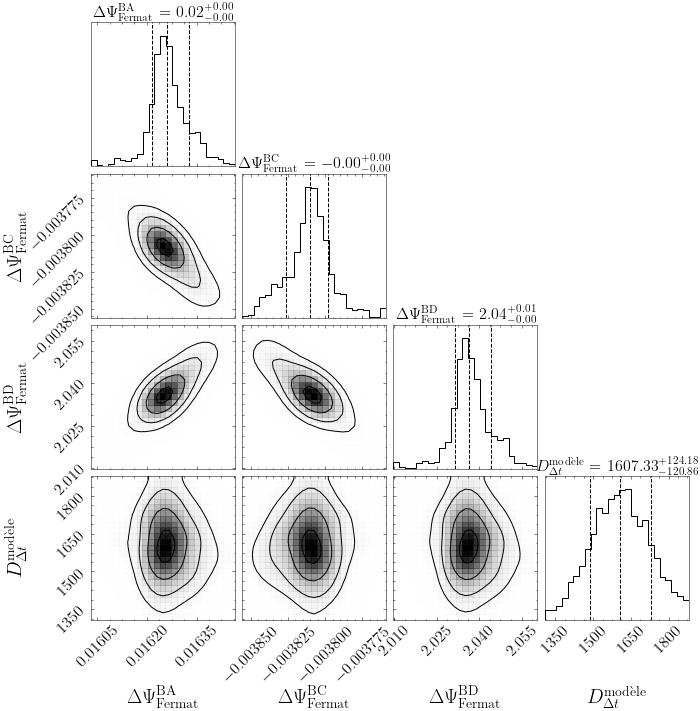
\includegraphics[width=\linewidth]{special_corner}
        \caption{Contraintes cosmographiques sur le système RXJ1131-1231. L'ajustement 
        d'un KDE est adoucie par un facteur de bande $h=2$. Les contours équivalents 
aux 16$^{e}$, 50$^{e}$ et 84$^{e}$ quantiles sont affichés sur 98\% de la masse des distributions 
jointes. Ces ajustements sont fait pour adoucir les modes \textit{pirates} provenants 
de chaînes MCMC qui n'ont pas atteint l'état ergodique.}
        \label{fig:special}
\end{figure}



On approxime la distribution postérieur de $D_{\Delta}^{\text{modèle}}$ par 
ses trois premiers moments pour estimer 
$D_{\Delta t}$ par l'équation \eqref{eq:Degenerescence}. C'est-à-dire qu'on pèse les 
échantillons MCMC de $D_{\Delta t}^{\text{modèle}}$ et les échantillons simulés 
de $\kappa_{\mathrm{ext}}$ par 
le produit de leur distribution respective (Pearson type III). Les 
paramètres cosmologiques $\Omega_m$ et $\Omega_\Lambda$ utilisés 
pour calculer les 
distances de diamètres angulaires (équation \eqref{eq:Ddt}) sont 
pris comme étant fixent et égal à leur valeur estimé par la \citet{PlanckCollaboration2018}. 
L'incertitude sur leur valeur n'a qu'un impact minimal sur la valeur de $H_0$ obtenu. 
Une étude plus détaillé de l'impact de la cosmologie sur la valeur de la constante de 
Hubble obtenu peut être trouvée dans l'article de \citet{Suyu2013} ainsi 
que la revue de \citet{Treu2010}. La distribution obtenue est présentée dans la figure 
\ref{fig:H0}.


\begin{figure}[H]
        \centering
        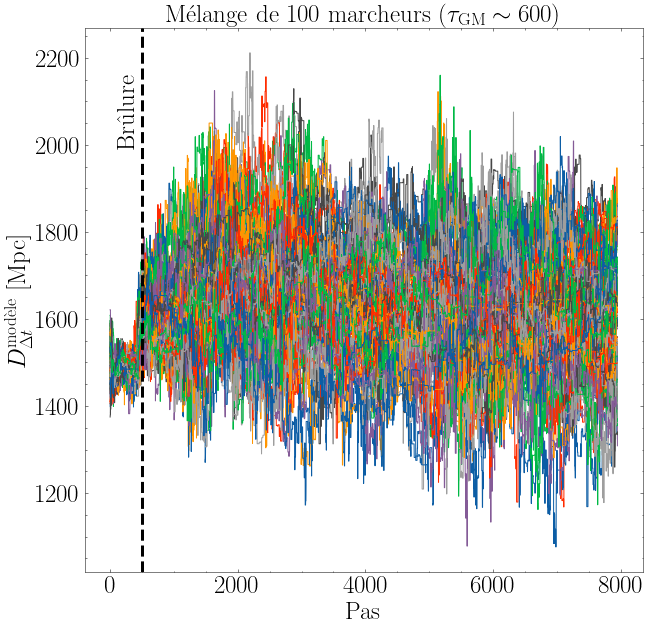
\includegraphics[width=\linewidth]{ddt_walkers_mixing}
        \caption{Chaînes MCMC des marcheurs projeté sur le paramètre 
        $D_{\Delta t}^{\text{modèle}}$. La brûlure réfère au pas où les données 
sont enregistrées pour déterminer la distribution \textit{a posteriori}. Les chaînes 
sont bien mélangées comme en témoigne l'inspection visuelle. Toutefois l'analyse de 
convergence échoue car les chaînes ne sont pas assez longues pour estimer le temps 
d'autocorrélation avec l'estimateur de \citet{Goodman2010}.}
        \label{fig:mixing}
\end{figure}



\begin{figure}[H]
        \centering
        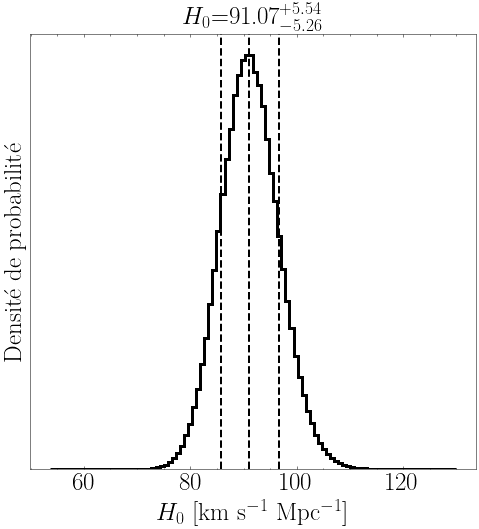
\includegraphics[width=0.8\linewidth]{H0_posterior}
        \caption{Distribution \textit{a posteriori} de la constante de Hubble 
        estimé avec $D_{\Delta t}$ et les paramètres cosmologiques de 
la \citet{PlanckCollaboration2018}. Les lignes verticales correspondes 
aux 16$^{e}$, 50$^{e}$ et 84$^{e}$ quantiles.}
        \label{fig:H0}
\end{figure}

Les distributions jointes et marginalisées des paramètres de la lentilles 
sont présentés dans la figure \ref{fig:cornerplot}. La médiane des distributions 
marginalisée et les incertitudes correspondant à $68\%$ de la masse 
sont présentées et comparées dans la table \ref{tab:results}. 

On note la différence de $2.1\sigma$ entre la valeur $D_{\Delta t}^{\text{modèle}}$ 
qu'on rapporte et celle rapportée par \citet{Suyu2013} (table \ref{tab:results}). 
Bien que cette différence ne 
soit pas statistiquement significative, il est intéressant de soulever que le 
biais observé par notre analyse pousse la distance caractéristique vers des valeurs 
plus petites (et donc inversement $H_0$ vers des valeurs plus grandes). Ce biais est aussi 
représenté par
%l'asymétrie négative 
%de la distribution marginalisé de $D_{\Delta t}^{\text{modèle}}$ 
%dans la figure \ref{fig:special} et 
l'asymétrie positive de la distribution 
marginalisée de $H_0$ (figure \ref{fig:H0}). 

On formule notre hypothèse sur la nature de ce biais en suivant l'analyse de 
\citet{Birrer2016} sur la dégénérescence de masse et l'importance de la modélisation 
de la cinématique stellaire. Les auteurs estiment que la distribution \textit{a priori} 
sur les paramètres du profil de \citet{Hernquist1990} est responsable d'environ 
7.5\% du budget d'erreur sur $H_0$, soit environ la taille du biais que nous observons 
entre la valeur déterminée par cette étude et la valeur rapportée par 
\citet{Suyu2013}. 

Notre estimé de la constante de Hubble $91.07^{+5.54}_{-5.26}$ (figure \ref{fig:H0})
atteint une précision de $6\%$ similaire à celle rapportée 
par \citet{Suyu2013}, soit $4.0\%$ pour leur estimé avec un univers $\Lambda$CDM. Puisqu'on 
fait des hypothèses simplificatrices pour le modèle du champ de convergence et le 
modèle de la source, on s'attend à ce que notre estimé de l'incertitude soit 
plus grande que celle rapportée par \citet{Suyu2013}. Il est très probable 
que notre étude surestime la précision puisque la vraisemblance modélisant la cinématique 
stellaire n'est pas prise en compte durant l'inférence des paramètres.

%Notre analyse introduit donc un biais statistique significatif du fait qu'on ne contraint 
%pas la cinématique stellaires durant l'inférence comme c'est accompli par 
%\citet{Suyu2013} et plus récemment par \citet{Birrer2016}.

\begin{figure*}[ht]
        \centering
        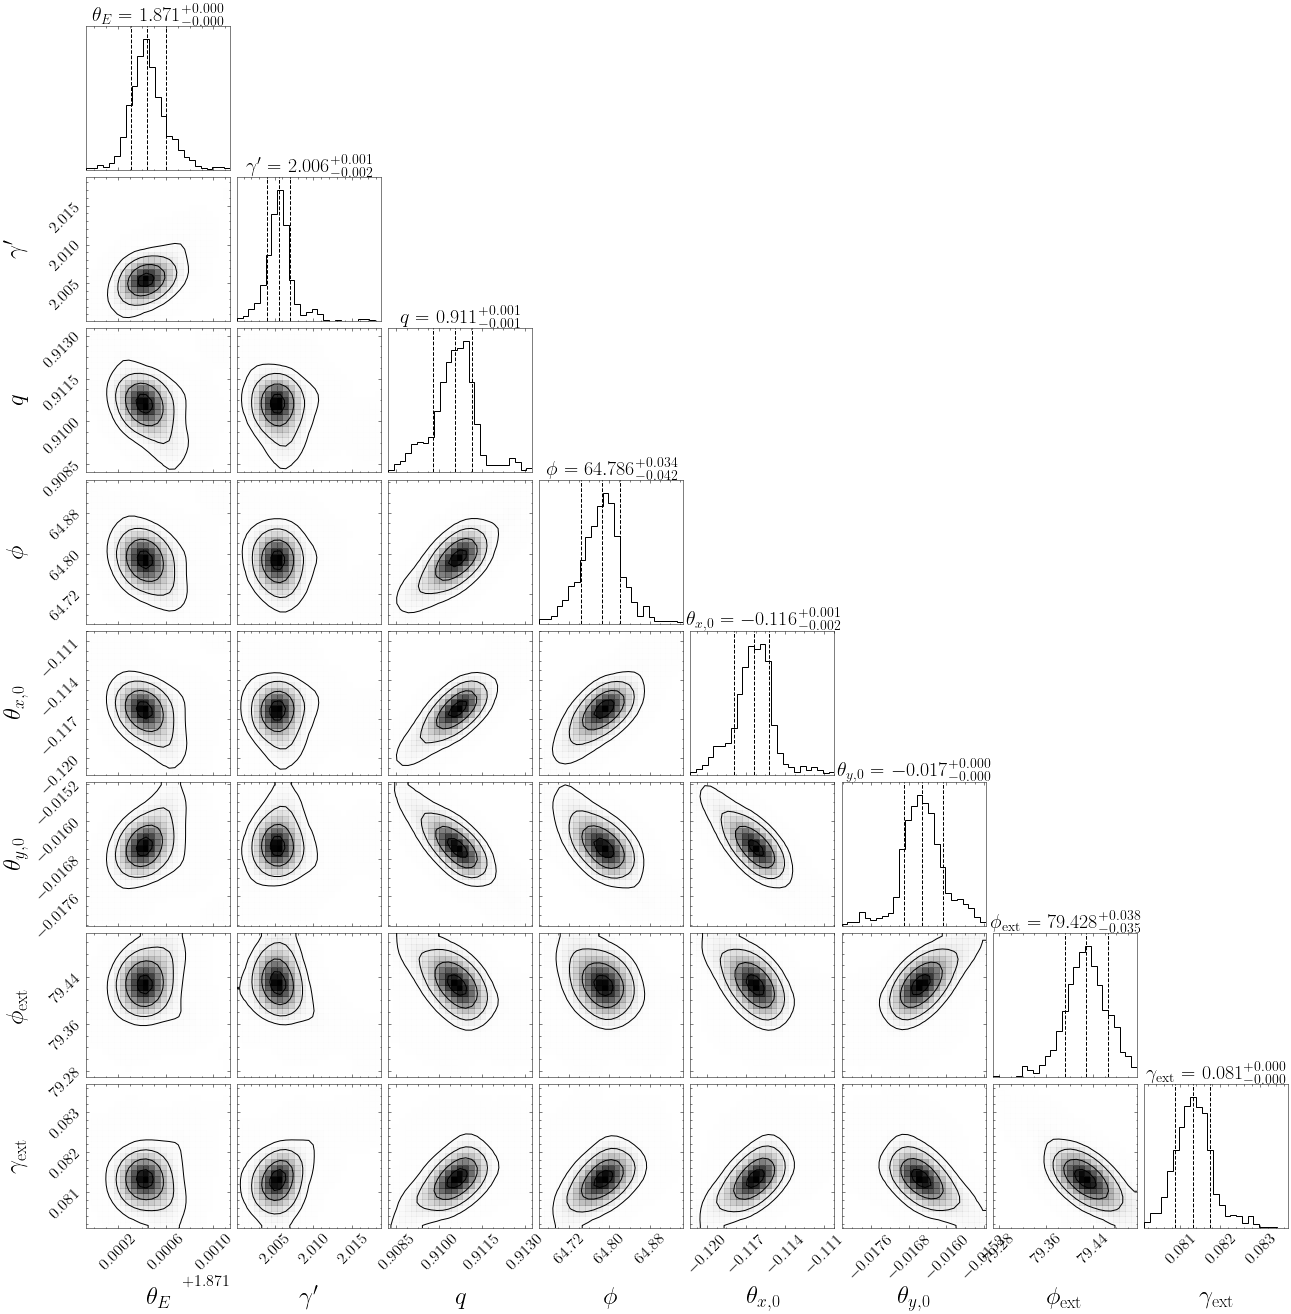
\includegraphics[width=\textwidth]{lens_params_corner_plot}
        \caption{}
        \label{fig:cornerplot}
\end{figure*}
\begin{table*}[hb]
        \centering
        \begin{tabular}{lcccc}
\toprule
\toprule
\thead{Description} & 
\thead{Paramètre} & \thead{Population initiale \\ (100 particules)} & 
\thead{Contrainte \\ marginalisée ou \\ optimisée}  & \thead{\citet{Suyu2013}} \\
\midrule
Distribution de masse la lentille 
\\\midrule
Rayon d'Einstein [arcsec] & 
        $\theta_E$ &$\mathcal{N}(1.5, 0.3)$ & 
        $1.8714^{+0.0002}_{-0.0001}$ & 
        $1.64^{+0.01}_{-0.02}$ \\[1ex]
Pente logarithmique & 
        $\gamma'$ & 
        $\mathcal{N}(2, 0.2)$ & 
        $2.005^{+0.002}_{-0.002}$ & 
        $1.95^{+0.01}_{-0.04}$ \\[1ex]
Ratio d'axe & 
        $q$ & 
        $\mathcal{N}_{e_i}(0.1, 0.1)$ & 
        $0.9106^{+0.0006}_{-0.0008}$ & 
        $0.763^{+0.005}_{-0.008}$ \\[1ex]
Orientation de l'axe principal [$^{\circ}$] & 
        $\phi$ & $\mathcal{U}(0, 360)$ &
        $64.78^{+0.03}_{-0.04}$ &
        \\[1ex]
Centre de masse en $\theta_x$ [arcsec] & 
        $\theta_{x, 0}$ & 
        $\mathcal{N}(0, 0.1)$ & 
        $-0.116^{+0.001}_{-0.002}$\\[1ex]
Centre de masse en $\theta_y$ [arcsec] &
        $\theta_{y, 0}$ & 
        $\mathcal{N}(0, 0.1)$ & 
        $-0.0165^{+0.0004}_{-0.0004}$\\[1ex]
Magnitude du cisaillement & $\gamma_{\mathrm{ext}}$ & 
        $\mathcal{N}_{\gamma_i}(0.01, 0.1)$ &
        $0.0813^{+0.0004}_{-0.0005}$ & 
        $0.089^{+0.006}_{-0.006}$ \\[1ex]
Orientation du cisaillement [$^{\circ}$]&  
        $\phi_{\mathrm{ext}}$ & 
        $\mathcal{U}(0, 360)$ &
        $79.428^{+0.038}_{-0.035}$\\[1ex]
\midrule
\multicolumn{2}{l}{Profils de Sérsic de G (Optimisé avec \texttt{GalFit}, $\chi^2=3.83$)}\\
\midrule
%Centre du disque en $\theta_1$ [arcsec] & 
%$\theta^{Gi1}_{x, 0}$ &&
            %$-0.03150 \pm 0.00001$       & 
            %\\[1ex]
%Centre du disque en $\theta_2$ [arcsec] & 
%$\theta^{G}_{y, 0}$ & &
        %$0.02329 \pm 0.00001$
        %\\[1ex]
%Centre du bulbe en $\theta_1$ [arcsec] & 
%$\theta^{Gi1}_{x, 0}$ &&
            %$-0.03150 \pm 0.00001$       & 
            %\\[1ex]
%Centre du bulbe en $\theta_2$ [arcsec] & 
%$\theta^{G}_{y, 0}$ & &
        %$0.02329 \pm 0.00001$
        %\\[1ex]
Ratio d'axe du disque & 
        $q_{G1}$ &
          --      & 
        $0.752 \pm 0.001$ & 
        $0.878^{+0.004}_{-0.003}$ \\[1ex]
Orientation du disque [$^{\circ}$] & 
        $\phi_{G1}$ &
          --      & 
        $-65.9 \pm 0.3$ & \\[1ex]
Indice de Sérsic du disque & 
        $n_{G1}$ &
            --    & 
        $3.94 \pm 0.03$ & 
        $0.93^{+0.03}_{-0.03}$ \\[1ex]
Rayon effectif du disque [arcsec] & 
        $R_{\mathrm{eff}, G1}$ &
              --                & 
        $5.27 \pm 0.09$ & 
        $2.49 \pm 0.01$ \\[1ex]
Ratio d'axe du bulbe & 
        $q_{G2}$ &
          --      &
        $0.856 \pm 0.004$ & 
        $0.849^{+0.004}_{-0.004}$ \\[1ex]
Orientation du bulbe [$^{\circ}$]& $\phi_{G2}$& 
           --     &
        $5.21 \pm1.4$ &
        \\[1ex]
Indice de Sérsic du bulbe & 
        $n_{G2}$ &
            --    & 
        $1.29 \pm 0.01$ & 
        $1.59^{+0.03}_{-0.03}$ \\[1ex]
Rayon effectif du bulbe [arcsec] & 
        $R_{\mathrm{eff}, G2}$ &
              --          & 
        $0.212 \pm 0.002$  & 
        $0.362 \pm 0.009$ \\[1ex]

%\midrule
%Profils de Sérsic de la source \\
%\midrule
\midrule
Paramètres de la source \\
\midrule
Position du quasar en $\theta_x$ [arcsec] & 
        $\beta_x^{\mathrm{AGN}}$ & 
           --     &
        $0.505^{+0.04}_{-0.04}$ & 
--        \\[1ex]
Position du quasar en $\theta_y$ [arcsec] & 
        $\beta_y^{\mathrm{AGN}}$ & 
             --                    &
        $-0.182^{+0.001}_{-0.001}$ &
  --      \\[1ex]
Rayon effectif du disque [arcsec] & 
        $R_{\mathrm{eff}, S1}$ & 
        $\mathcal{N}(1, 0.1)$ & 
        $0.105^{+0.001}_{-0.001}$ & 
    --    \\[1ex]
Indice de Sérsic du disque & 
        $n_{S1}$ & 
        $\mathcal{N}(1, 0.5)$ & 
        $0.562^{+0.01}_{-0.009}$ & 
      --  \\[1ex]
Ratio d'axe du disque & 
        $q_{S1}$ & 
        $\mathcal{N}_{e_i}(0, 0.2)$ & 
        $0.791^{+0.005}_{-0.005}$ &
 --       \\[1ex]
Orientation du disque [$^{\circ}$]&
        $\phi_{S1}$ & 
        $\mathcal{U}(0, 360)$ & 
        $-14.9^{+1}_{-0.8}$ & 
   --     \\[1ex]
Rayon effectif du bulbe [arcsec] & 
        $R_{\mathrm{eff}, S2}$ & 
        $\mathcal{N}(1, 0.1)$ & 
        $0.838^{+0.007}_{-0.007}$ & 
    --    \\[1ex]
Indice de Sérsic du bulbe & 
        $n_{S2}$ & 
        $\mathcal{N}(1, 0.5)$ & 
        $0.5$ & 
    --    \\[1ex]
Ratio d'axe du bulbe & 
        $q_{S2}$ & 
        $\mathcal{N}_{e_i}(0, 0.2)$ & 
        $0.461^{+0.003}_{-0.003}$ &
     --   \\[1ex]
Orientation du bulbe [$^{\circ}$]&
        $\phi_{S2}$ & 
        $\mathcal{U}(0, 360)$ & 
        $-32.6^{+0.1}_{-0.1}$ & 
     --   \\[1ex]
\midrule
Paramètre cosmographique \\
\midrule
Distance caractéristique du délai temporel [Mpc]& 
        $D_{\Delta t}^{\text{modèle}}$ & 
        $\mathcal{U}(500, 10^4)$ & 
        $1631^{+116}_{-115}$ & 
        $1883^{+89}_{-85}$\\[1ex]
\bottomrule
\bottomrule
        \end{tabular}
        \caption{Paramètres optimisées et marginalisés du système RXJ1131-1231.}
        \label{tab:results}
\end{table*}


\section{Conclusion}\label{sec:conclusion}
Nous avons performer une reconstruction paramétrique des profils de lumières 
des galaxies G et S et de la source lentillé, ainsi qu'une reconstruction paramétrique 
d'un champ de convergence elliptique à loi de puissance adoucie pour estimer les 
potentiels de Fermat qui donnent lieu aux 4 images du quasar dans l'image du télescope 
Hubble du système RXJ1131-1231.

Combiné avec l'estimé des délais temporels et de la masse dans la ligne de visée 
$\kappa_{\mathrm{ext}}$, nous avons fourni un estimé de la constante de Hubble 
$H_0 = 91.07^{+5.54}_{-5.26}$ avec une incertitude statistique estimé à 6\%. 
La valeur rapportée diffère de celle rapportée par \citet{Suyu2013} par $2.1\sigma$, 
ce qui soulève le besoin d'estimer les incertitudes systématiques dans notre analyse 
et de modéliser la cinématique stellaire du système.


\printbibliography

\end{document}

